\documentclass[11pt]{article}

% ---------------------------------------------------------------------------
% Draft scientific article. Author names and affiliations are PLACEHOLDERS.
% Compile with: pdflatex ect_tensor_strain.tex  (run twice for references).
% ---------------------------------------------------------------------------

\usepackage[a4paper,margin=1in]{geometry}
\usepackage{amsmath,amssymb}
\usepackage{bm}
\usepackage{graphicx}
\usepackage{booktabs}
\usepackage{caption}
\usepackage[hidelinks]{hyperref}

\graphicspath{{figures/}}

\newcommand{\dsig}{\Delta\sigma}
\newcommand{\eps}{\bm{\varepsilon}}
\newcommand{\sig}{\bm{\sigma}}
\newcommand{\Kt}{\mathsf{K}}

\title{\textbf{Towards Tensorial Strain Reconstruction from\\
Eddy-Current Testing in Laser Powder Bed Fusion}}

\author{M.\ Carraturo\thanks{Corresponding author. Affiliations are placeholders
in this draft.}\quad B.\,I.\ Ates\\[2pt]
\small University of Pavia / Technical University of Munich (draft)}

\date{\today}

\begin{document}
\maketitle

\begin{abstract}
Eddy-current testing (ECT) is an attractive in-situ probe for laser powder bed
fusion (LPBF) because it is non-contact, fast, and sensitive to the electrical
conductivity, which depends on mechanical strain. Prior work established a
\emph{scalar} relation $\dsig/\sigma_0=\kappa\,\varepsilon$ between the relative
conductivity change and the strain, calibrated to $\kappa=-0.326$ for 316L
stainless steel. However, the residual strain in an as-built part is a
second-order \emph{tensor}, whereas a coil measures a single scalar impedance:
the reconstruction of a six-component tensor from scalar data is fundamentally
under-determined. We present a framework that resolves this tension by combining
(i) a tensorial elastoresistivity model that generalises $\kappa$ to a
fourth-order coupling tensor; (ii) a finite-element (FEM) reciprocity analysis
that quantifies which conductivity components a given probe senses; (iii) an
optimal-design procedure for directional-probe sets (a conductivity ``rosette'');
and (iv) a regularised, prior-informed inversion that fuses the measurements with
a thermomechanical process simulation (data assimilation). Along the way,
cross-validating the analytical model against the FEM --- whose impedance we
verify against an independent ohmic-loss balance to better than $10^{-5}$ ---
exposed two implementation pitfalls in our realisation of the classical
Dodd--Deeds model: a reflection-coefficient sign and a units error in the
propagation parameter. Such forward-model bugs survive a self-consistent
synthetic round trip (an inverse crime) but are caught by a dissimilar redundant
model; after correction the analytical and FEM normalised impedances agree to
$0.9\%$ in resistance and $2.8\%$ in reactance. On synthetic LPBF builds, a single normal coil
resolves one strain degree of freedom, an in-plane rosette resolves three, and a
six-direction tilted set resolves all six; the prior supplies the components that
the probes cannot observe. The complete workflow is implemented in an open
pipeline that outputs a full strain-tensor field.
\end{abstract}

\section{Introduction}
Residual stress and strain are central concerns in metal additive manufacturing:
they drive distortion, cracking, and premature failure. In-situ monitoring that
could map the evolving strain field during a build would enable closed-loop
process control. Eddy-current testing (ECT) is a promising modality
\cite{garcia2011}: a coil driven at frequency $\omega$ induces eddy currents in
the conductive part, and the resulting change in coil impedance encodes the local
electrical conductivity $\sigma$. Because $\sigma$ depends on strain through the
elastoresistive effect, ECT indirectly senses strain.

The thesis underlying this work \cite{ates2025} established two pillars: (a)
reconstruction of as-built geometry from ECT data for immersed-boundary (finite
cell) simulation, and (b) a calibrated \emph{scalar} law
\begin{equation}
  \frac{\dsig}{\sigma_0} = \kappa\,\varepsilon, \qquad \kappa = -0.326
  \;\; (\text{316L}),
  \label{eq:scalar}
\end{equation}
with coefficient of determination $R^2=0.992$ in uniaxial tension. Equation
\eqref{eq:scalar} is, however, a one-dimensional projection of a richer physical
reality. In three dimensions the strain $\eps$ is a symmetric second-order tensor
with six independent components, while a coil reports a single scalar. Recovering
six numbers from one is impossible without additional information.

\paragraph{Related work.} That conductivity depends on elastic strain through the
piezoresistive (elastoresistive) effect underpins an established line of
eddy-current residual-stress assessment developed largely by the Nagy group:
high-frequency apparent-conductivity spectroscopy and iterative inversion recover
near-surface residual-stress depth profiles in shot-peened superalloys
\cite{yu2004,abunabah2006,abunabah2007}. That work also established a key
confounder --- cold work and dislocation-density changes alter conductivity
alongside elastic strain --- which is especially pronounced in LPBF
microstructures and which we revisit in Section~\ref{sec:feasibility}. In metal
additive manufacturing, recoater-mounted ECT is already used for layer-wise
density and defect monitoring \cite{spurek2022,monu2025}, with part-temperature
compensation shown to be essential \cite{spurek2024}; residual stress is a
central concern of the field \cite{bartlett2019,withers2001} but is not yet mapped
in~situ.
Our contribution is therefore not ``ECT senses strain'' but a \emph{tensorial}
observability framework, optimal rosette design, and simulation-prior fusion that
together target the strain \emph{tensor} in LPBF.

This paper develops the methodology and tooling to close that gap. We make four
contributions: a tensorial elastoresistivity model (Section~\ref{sec:tensor}); an
FEM-based observability analysis (Section~\ref{sec:obs}) built on a forward model
that we verify and cross-validate (Section~\ref{sec:forward}); an optimal
directional-probe (``rosette'') design
(Section~\ref{sec:design}); and a prior-informed tensor inversion realised inside
an integrated pipeline (Sections~\ref{sec:inv}--\ref{sec:pipeline}).

\section{Forward model and validation}
\label{sec:forward}

\subsection{Analytical Dodd--Deeds model}
For a cylindrical multi-turn coil of inner/outer radius $r_i,r_o$, length $\ell$,
$n$ turns and lift-off $s$ above a conductive half-space, the impedance follows
the Dodd--Deeds formulation \cite{dodd1968,bowler2019,theodoulidis2006}
\begin{equation}
  Z = \frac{\mathrm{j}\omega\mu_0\pi n^2}{\ell^2 (r_o-r_i)^2}
  \int_0^\infty \frac{J^2(\alpha r_i,\alpha r_o)}{\alpha^5}
  \Big[\,2\ell + \tfrac{1}{\alpha}\big(2e^{-\alpha\ell}-2 + P(\alpha)\,\Gamma(\alpha)\big)\Big]\,
  \mathrm{d}\alpha,
  \label{eq:dd}
\end{equation}
where $P(\alpha)=e^{-2\alpha(\ell+s)}+e^{-2\alpha s}-2e^{-\alpha(\ell+2s)}$,
$\gamma=\sqrt{\alpha^2+\mathrm{j}\omega\mu\sigma}$ and $\Gamma$ is the half-space
reflection coefficient; $J(\alpha r_i,\alpha r_o)=\int_{\alpha r_i}^{\alpha r_o}
x\,J_1(x)\,\mathrm{d}x$ is the coil's Bessel kernel and $\mu=\mu_0$ for the
non-magnetic 316L considered here. The normalised impedance is
$Z_{\mathrm{norm}}=(Z_0-Z)/\operatorname{Im}(Z_0)$ with $Z_0$ the free-space
(self) impedance.

The physically correct reflection coefficient for a non-magnetic half-space is
\begin{equation}
  \Gamma(\alpha)=\frac{\alpha-\gamma}{\alpha+\gamma},
  \label{eq:refl}
\end{equation}
which tends to $-1$ as $\sigma\to\infty$: eddy currents then reduce the net
inductance and add resistance, as required physically. A realisation that uses
the opposite sign, $(\gamma-\alpha)/(\alpha+\gamma)$, predicts the unphysical
opposite (increasing reactance, negative resistance over a passive conductor).
This pitfall is invisible to a self-consistent synthetic round trip --- an
\emph{inverse crime} --- but corrupts the inversion of real data; we caught it
only by cross-validating against the dissimilar FEM model below.

\subsection{Axisymmetric finite-element model}
To handle geometries where the half-space assumption fails (finite parts, layers,
defects), we solve the time-harmonic eddy-current problem for the azimuthal
magnetic vector potential $A_\phi$ in axisymmetric coordinates:
\begin{equation}
  \frac{1}{\mu}\!\int\!\Big[\nabla A_\phi\!\cdot\!\nabla v
  + \frac{A_\phi v}{\rho^2}\Big]\rho\,\mathrm{d}\rho\,\mathrm{d}z
  + \mathrm{j}\omega\!\int\!\sigma A_\phi v\,\rho\,\mathrm{d}\rho\,\mathrm{d}z
  = \int J_s\, v\,\rho\,\mathrm{d}\rho\,\mathrm{d}z,
  \label{eq:weak}
\end{equation}
with $A_\phi=0$ on the symmetry axis and the truncated outer boundary. The coil
impedance is obtained from the flux linkage of the winding,
\begin{equation}
  \Lambda = \frac{n}{S_{\mathrm{coil}}}\!\iint_{\mathrm{coil}}\! 2\pi\rho\,A_\phi\,
  \mathrm{d}\rho\,\mathrm{d}z, \qquad Z=\mathrm{j}\omega\Lambda/I,
  \label{eq:flux}
\end{equation}
and $Z_0$ is computed by the same model with $\sigma=0$, giving a self-consistent
normalisation.

\begin{table}[t]
\centering
\caption{FEM forward-model results and internal-consistency (verification)
checks (reference coil over a generic conductor, $\sigma=16.2$~MS/m, $240$~kHz;
realistic 316L values are used in Section~\ref{sec:feasibility}).}
\label{tab:fem}
\begin{tabular}{lll}
\toprule
Quantity & Value & Check\\
\midrule
$Z_0$ (coil in air)        & $0 + 5.18\times10^4\,\mathrm{j}\;\Omega$ & purely inductive\\
$Z$ (over conductor)       & $622 + 3.73\times10^4\,\mathrm{j}\;\Omega$ & $\mathrm{Re}>0$, $\mathrm{Im}<\mathrm{Im}\,Z_0$\\
$\mathrm{Re}(Z)$ flux linkage & $622.35\,\Omega$ & --\\
$R$ from ohmic loss        & $622.35\,\Omega$ & agree to $<10^{-5}$\\
mesh convergence           & order 3 $\approx$ order 4 & 5 significant figures\\
\bottomrule
\end{tabular}
\end{table}

The FEM is mesh-converged and internally consistent: the resistance extracted
from the flux-linkage impedance \eqref{eq:flux} equals a direct volume integral
of the ohmic loss $\tfrac12\!\int\sigma|E|^2\,\mathrm{d}V$ to better than
$10^{-5}$ (Table~\ref{tab:fem}) --- a \emph{verification} check, distinct from
experimental validation. Cross-validating the analytical model against this FEM
exposed a second implementation pitfall in our realisation: a units error in the
propagation parameter $\gamma$ (a missing factor of $\mu_0$, so that
$\omega\mu\sigma$ no longer had units of $\mathrm{m}^{-2}$), which made the
conductor appear nearly perfect ($\Gamma\!\to\!-1$) --- an essentially correct
reactance but a loss suppressed by nearly three orders of magnitude. With both
the reflection sign \eqref{eq:refl} and the units corrected, the analytical and
FEM \emph{normalised} impedances agree to $0.9\%$ in resistance and $2.8\%$ in
reactance (Fig.~\ref{fig:fem}); the small reactance residual is the finite FEM
truncation versus the analytical half-space. The analytical integral
\eqref{eq:dd} is converged for $k_{\max}\!\sim\!6000$, within a stable plateau
before the oscillatory Bessel kernel degrades the quadrature. This benchmark uses
a reference coil over a generic conductor; realistic 316L parameters and their
resolution implications are treated in Section~\ref{sec:feasibility}.

\begin{figure}[t]
\centering
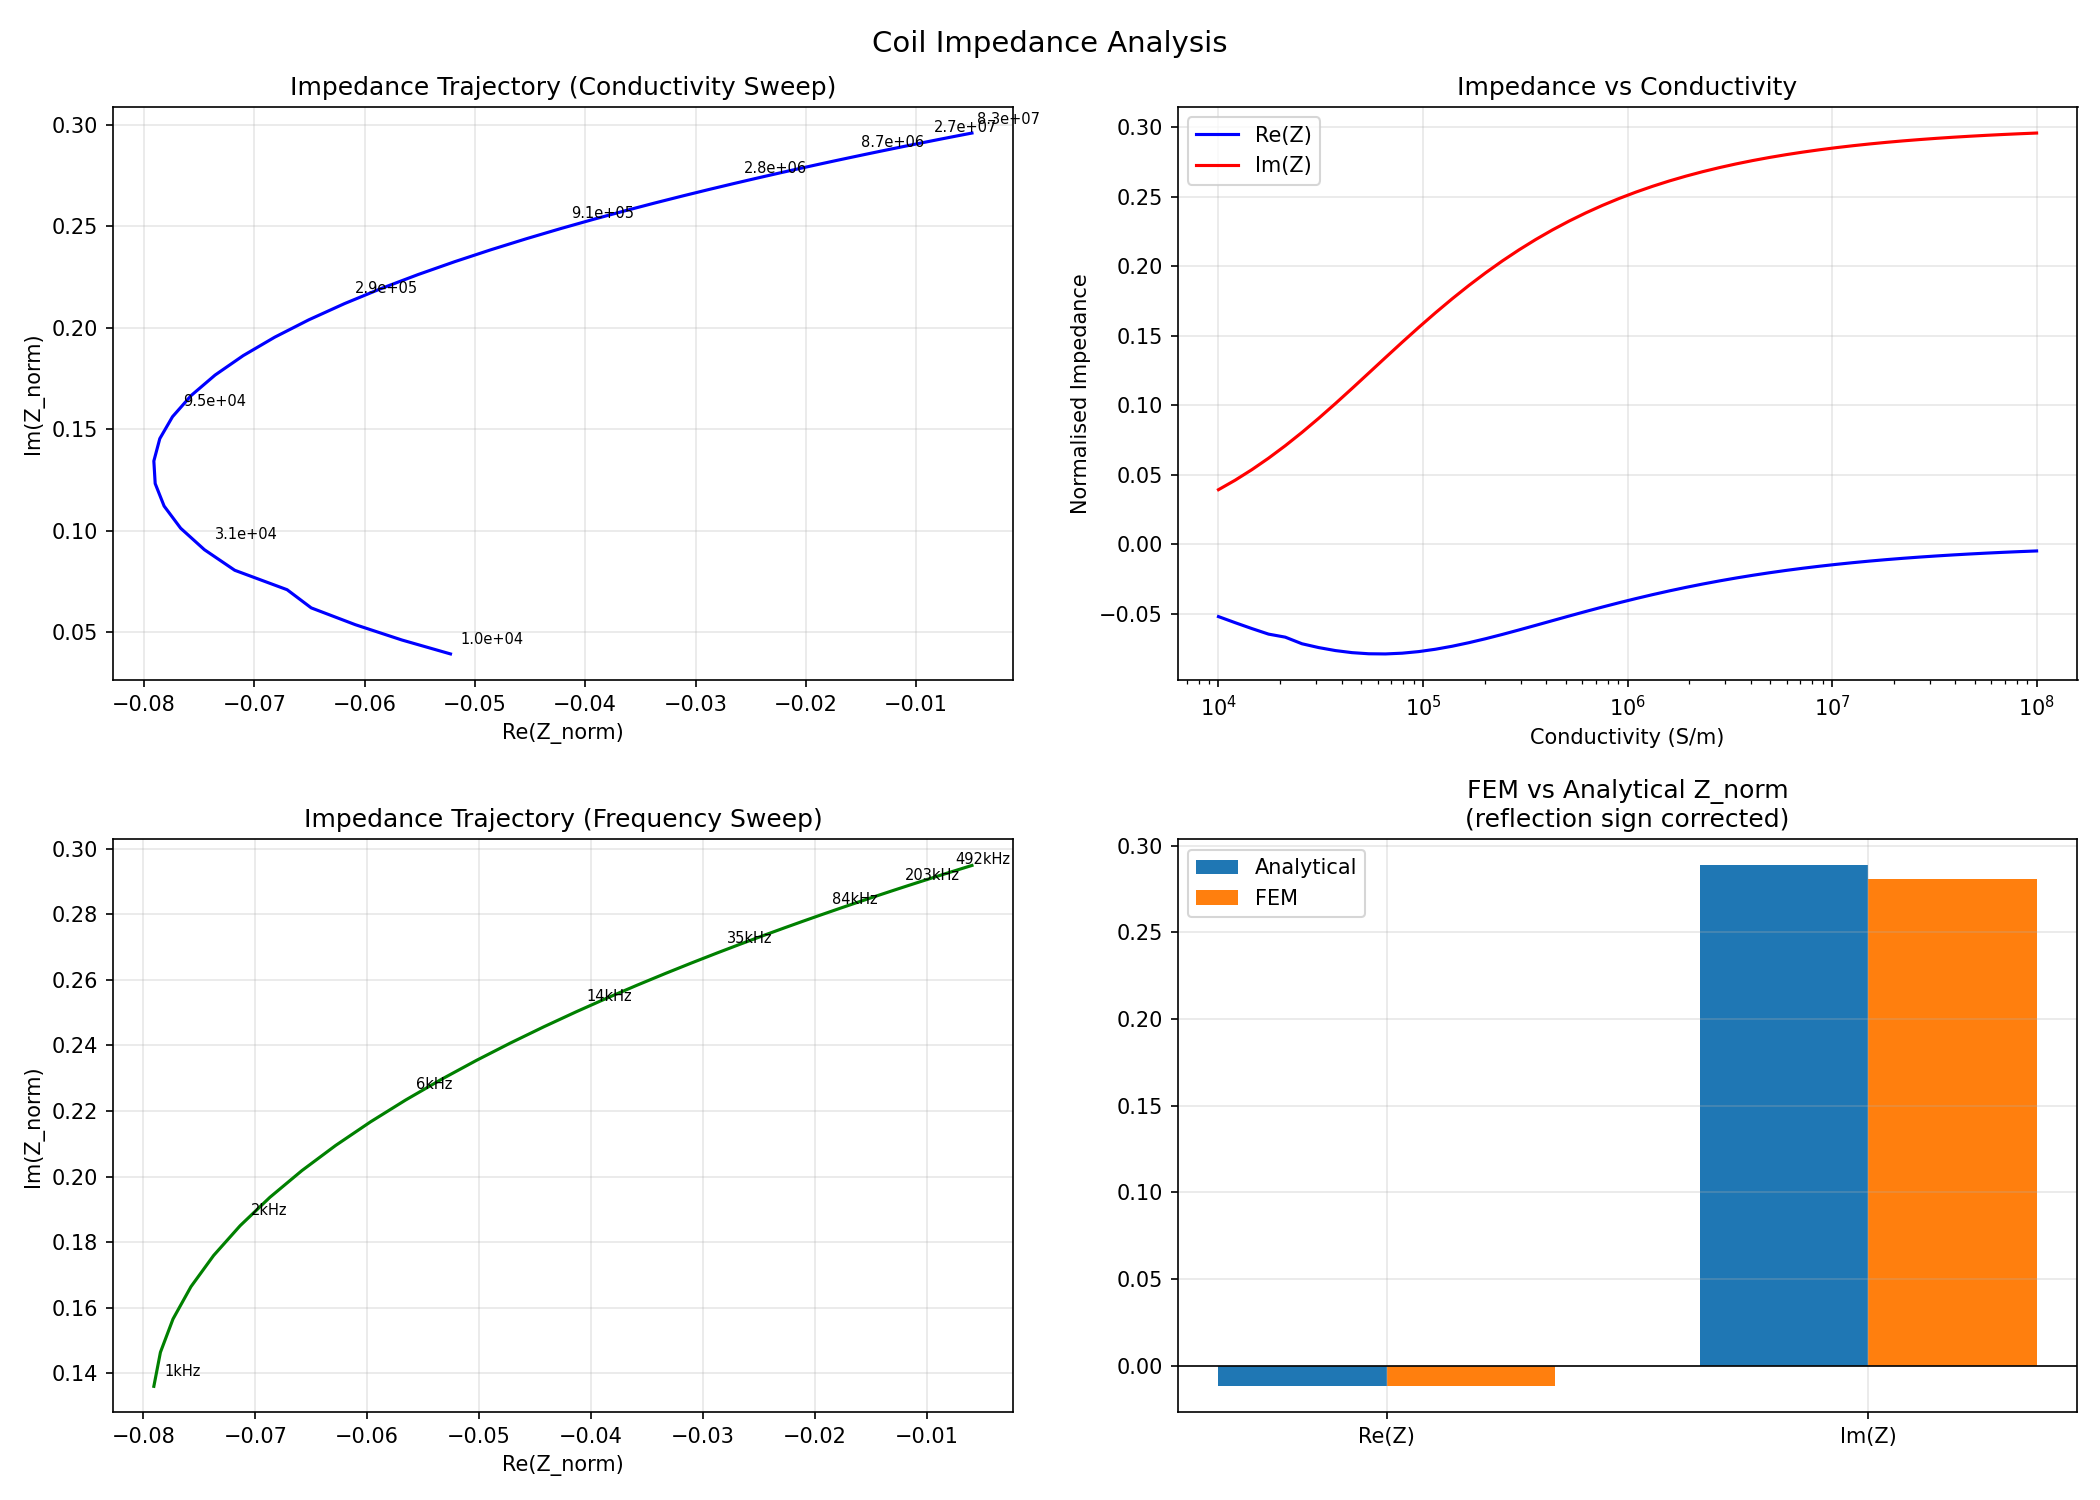
\includegraphics[width=0.92\textwidth]{fem_impedance_demo.png}
\caption{Coil impedance analysis. Analytical conductivity- and frequency-sweep
trajectories (top, bottom-left) and the FEM-vs-analytical normalised impedance
(bottom-right). After correcting the reflection sign and a units error in the
propagation parameter, the FEM and analytical normalised impedances agree in
both resistance ($0.9\%$) and reactance ($2.8\%$).}
\label{fig:fem}
\end{figure}

\section{From scalar to tensor: elastoresistivity}
\label{sec:tensor}
Strain breaks the isotropy of the material, so under load the conductivity is a
second-order tensor $\sigma_{ij}$ that couples to strain through a fourth-order
\emph{elastoresistivity} tensor $\Kt$:
\begin{equation}
  \frac{\dsig_{ij}}{\sigma_0} = K_{ijkl}\,\varepsilon_{kl}.
  \label{eq:tensor}
\end{equation}
For an isotropic base material $\Kt$ has the isotropic form
$K_{ijkl}=a\,\delta_{ij}\delta_{kl}+b(\delta_{ik}\delta_{jl}+\delta_{il}\delta_{jk})$,
i.e.\ two independent constants. Parameterising them as a longitudinal
$\kappa_\parallel$ and a transverse $\kappa_\perp$ coefficient,
\begin{equation}
  \frac{\dsig_{ii}}{\sigma_0}=\kappa_\parallel\varepsilon_{ii}
  + \kappa_\perp\!\!\sum_{k\neq i}\varepsilon_{kk}, \qquad
  \frac{\dsig_{ij}}{\sigma_0}=(\kappa_\parallel-\kappa_\perp)\varepsilon_{ij}
  \;\; (i\neq j).
\end{equation}
The scalar law \eqref{eq:scalar} is the uniaxial projection of \eqref{eq:tensor}:
the relative conductivity change sensed along a unit direction $\hat{\bm n}$ in a
uniaxial-stress test is $\hat{\bm n}^{\!\top}(\dsig/\sigma_0)\hat{\bm n}$, which
varies strongly with $\hat{\bm n}$ (Fig.~\ref{fig:tensor}). The measured value
$-0.326$ is therefore one directional projection, not a material invariant;
separating $\kappa_\parallel$ and $\kappa_\perp$ requires loading along several
orientations. A purely volumetric response ($\kappa_\parallel=\kappa_\perp$)
reduces $\Kt$ to rank one, so conductivity then constrains only the volumetric
strain $\operatorname{tr}\eps$.

\paragraph{Constants and provenance.} The elastoresistivity constants are not yet
independently calibrated; we anchor them to the available data. A single uniaxial
test fixes only one projection, so we choose $\kappa_\parallel$ such that the
along-load uniaxial projection reproduces the thesis scalar
($\kappa_\parallel-2\nu\kappa_\perp=-0.326$ at $\nu=0.30$), giving
$\kappa_\parallel=-0.374$ for an illustrative $\kappa_\perp=-0.08$. The result
figures use the round value $\kappa_\parallel=-0.40$ (along-load projection
$-0.352$, within $8\%$ of $-0.326$). Separating $\kappa_\parallel$ from
$\kappa_\perp$ requires multi-orientation loading (Section~\ref{sec:feasibility}).
Crucially, the observability results depend on these constants only through the
ratio $\kappa_\perp/\kappa_\parallel$, shown to be robust across its plausible
range in Section~\ref{sec:design}.

\begin{figure}[t]
\centering
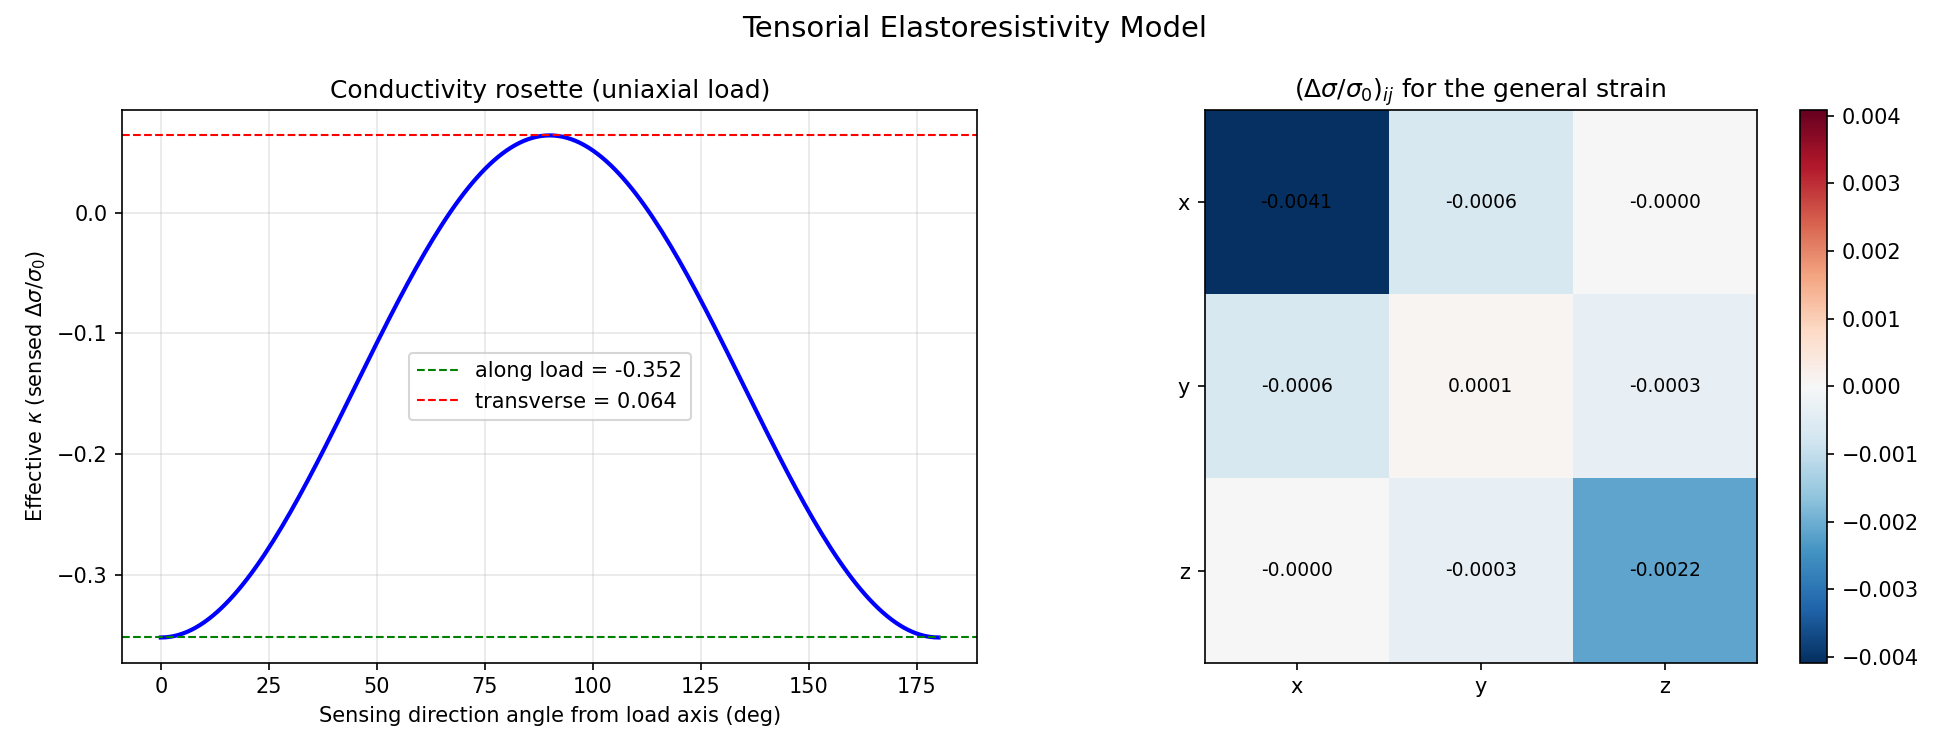
\includegraphics[width=0.92\textwidth]{tensor_model_demo.png}
\caption{Tensorial elastoresistivity. Left: the ``conductivity rosette'' --- the
effective $\kappa$ sensed in a uniaxial test depends on the sensing angle,
swinging from $-0.35$ (along load) to $+0.06$ (transverse). Right: the induced
$(\dsig/\sigma_0)_{ij}$ tensor for the strain $\varepsilon_{xx}=1.0\%$,
$\varepsilon_{yy}=-0.3\%$, $\varepsilon_{zz}=0.4\%$, $\varepsilon_{xy}=0.2\%$,
$\varepsilon_{yz}=0.1\%$ (illustrative $\kappa_\parallel=-0.40$,
$\kappa_\perp=-0.08$).}
\label{fig:tensor}
\end{figure}

\section{Observability analysis}
\label{sec:obs}

\subsection{Reciprocity sensitivity kernel}
By driving-point reciprocity \cite{auld1999}, a small conductivity perturbation
changes the coil impedance by
\begin{equation}
  \delta Z = -\frac{1}{I^2}\int \delta\sigma\, \bm E\!\cdot\!\bm E \,\mathrm{d}V.
  \label{eq:recip}
\end{equation}
For the axisymmetric coil the field is purely azimuthal,
$\bm E=-\mathrm{j}\omega A_\phi\,\hat{\bm\phi}$, so $\bm E\!\cdot\!\bm E=E_\phi^2$
and only the local azimuthal (in-plane) component of a tensor perturbation is
sensed. We confirmed \eqref{eq:recip} against finite-difference re-solves on a
fixed mesh, with the ratio approaching unity as the perturbation shrinks
($0.9963$ at $0.5\%$). Consequently a normal coil senses only in-plane
conductivity and is structurally \emph{blind} to $\sigma_{zz}$; its sensitivity
is concentrated within a skin depth of the surface (Fig.~\ref{fig:obs}, top-left).

\subsection{Directional probes and the conductivity rosette}
A directionally selective probe senses, to leading order, the effective
conductivity along its sensing direction,
\begin{equation}
  y(\hat{\bm n}) = \hat{\bm n}^{\!\top}\sig\,\hat{\bm n},
  \label{eq:proj}
\end{equation}
the conductivity analogue of a mechanical strain-gauge rosette.

Equation~\eqref{eq:proj} is a leading-order model: it assumes each probe drives
current cleanly along $\hat{\bm n}$. Accessed from the build surface this is well
justified in-plane but optimistic out-of-plane, because the induced eddy currents
are confined within a skin depth and flow essentially parallel to the surface ---
the axisymmetric solve of Section~\ref{sec:forward} makes this exact, with $\bm E$
purely azimuthal so that a normal coil is rigorously blind to $\sigma_{zz}$. A
coil merely tilted above the surface therefore gains only limited $\sigma_{zz}$
sensitivity; genuine out-of-plane access calls for edge/side probing, elongated or
rotating-field probes, or multi-frequency depth profiling. We accordingly treat
the six-direction, full-rank result below as an \emph{upper bound} on what
directional diversity can deliver, and take the in-plane rosette combined with the
simulation prior (Section~\ref{sec:inv}) as the practical configuration;
extracting the true out-of-plane row of $\mathsf M$ from a 3-D anisotropic
eddy-current model is left to future work.

Stacking $M$ probes gives a linear map
$\bm y = \mathsf{M}\,\bm\sigma_{\mathrm{v}}$ from the conductivity Voigt vector to
the measurements; composing with $\Kt$ yields the
strain map $\bm y = \mathsf{A}\,\eps_{\mathrm v}$ with
$\mathsf{A}=\sigma_0\,\mathsf{M}\,\Kt$. The singular value decomposition of
$\mathsf A$ gives the number of resolvable strain combinations (rank), their
conditioning, and the null space (blind directions). Table~\ref{tab:obs}
summarises the resolving power of representative configurations.

\begin{table}[t]
\centering
\caption{Resolvable strain degrees of freedom and conditioning by probe set. The
tilted six-probe row presumes idealised out-of-plane access and is an upper bound
(Section~\ref{sec:obs}).}
\label{tab:obs}
\begin{tabular}{lcc}
\toprule
Configuration & resolvable DOF (of 6) & condition number\\
\midrule
Single normal coil          & 1 & 1.0\\
In-plane rosette (0/45/90)   & 3 & 2.6\\
In-plane rosette (0/60/120)  & 3 & 2.2\\
Optimised in-plane rosette   & 3 & 1.9\\
Rosette + tilted probes (6)  & 6 & 2.5\\
\bottomrule
\end{tabular}
\end{table}

\begin{figure}[t]
\centering
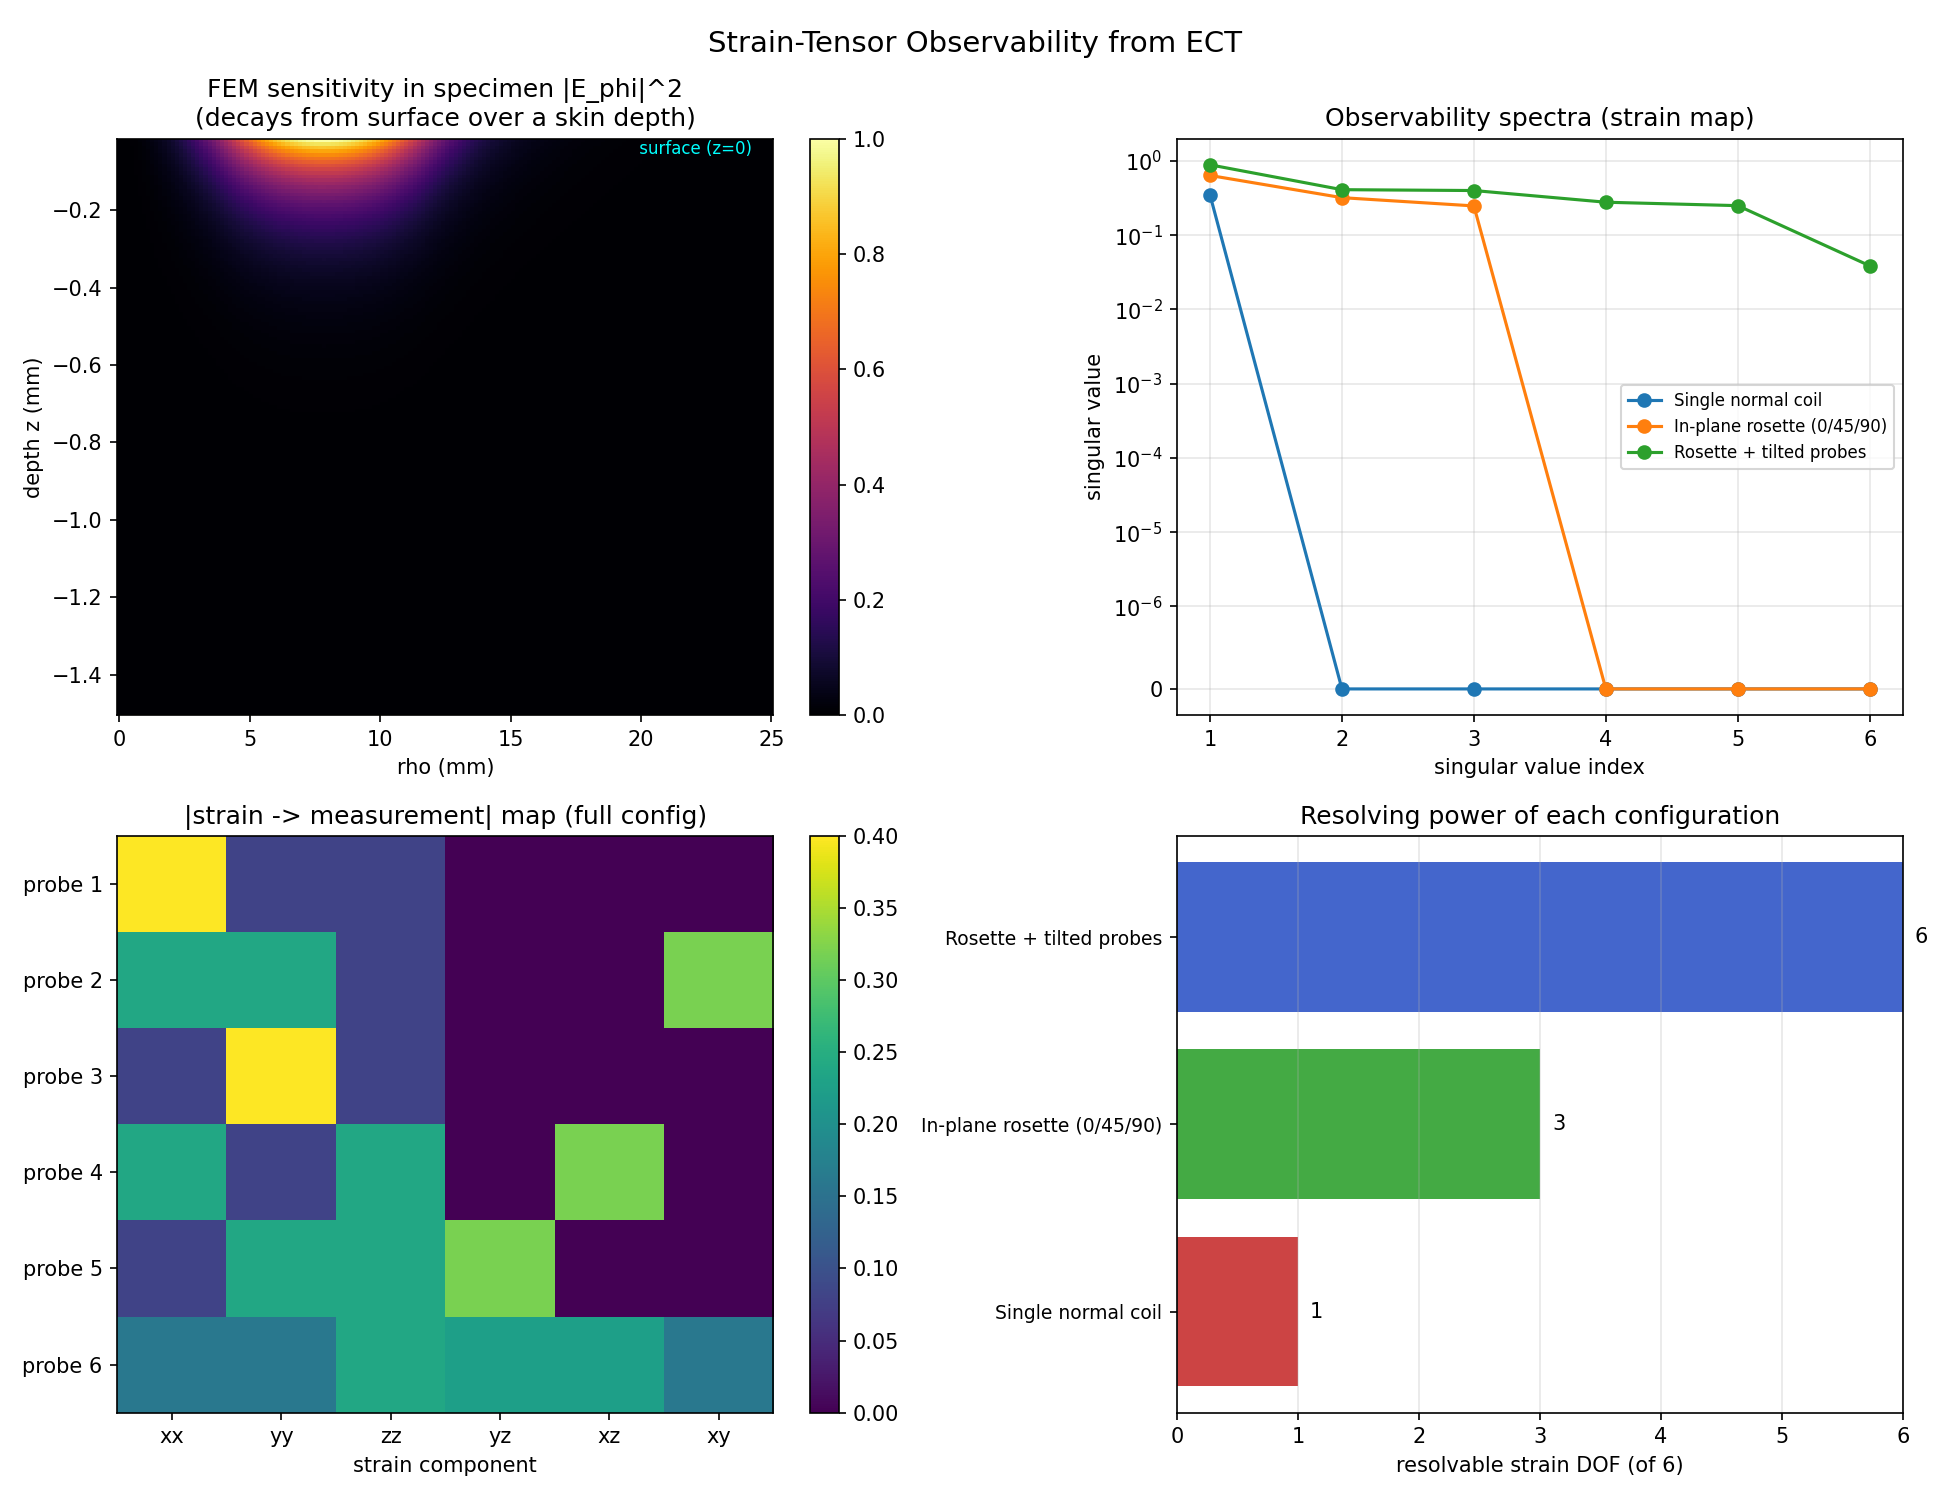
\includegraphics[width=0.92\textwidth]{observability_demo.png}
\caption{Observability. Top-left: FEM sensitivity density $|E_\phi|^2$ in the
specimen, decaying from the surface over a skin depth. Remaining panels: SVD
spectra, strain-to-measurement map, and resolving power of the normal coil
(1 DOF), in-plane rosette (3 DOF) and full tilted set (6 DOF).}
\label{fig:obs}
\end{figure}

\section{Probe-configuration design}
\label{sec:design}
Given $\Kt$ and the model \eqref{eq:proj}, we choose sensing directions that make
the inversion full-rank and well-conditioned by minimising the condition number
of $\mathsf A$ subject to a rank constraint. For three in-plane probes the
optimiser improves on the naive $0/45/90$ ($\mathrm{cond}=2.57$) and the delta
rosette $0/60/120$ ($2.18$), reaching $1.93$. A six-direction set that includes
tilted probes attains full rank ($6$) at $\mathrm{cond}=2.50$
(Fig.~\ref{fig:design}) --- an upper bound that presumes the idealised
out-of-plane access discussed in Section~\ref{sec:obs}. The ceiling is set by $\operatorname{rank}\Kt$: directional
diversity helps only insofar as the elastoresistive response is anisotropic.
Excitation frequency provides a complementary, depth-selective degree of freedom
through the skin depth $\delta=\sqrt{2/(\omega\mu\sigma)}$
(Fig.~\ref{fig:design}, bottom-right).

\begin{figure}[t]
\centering
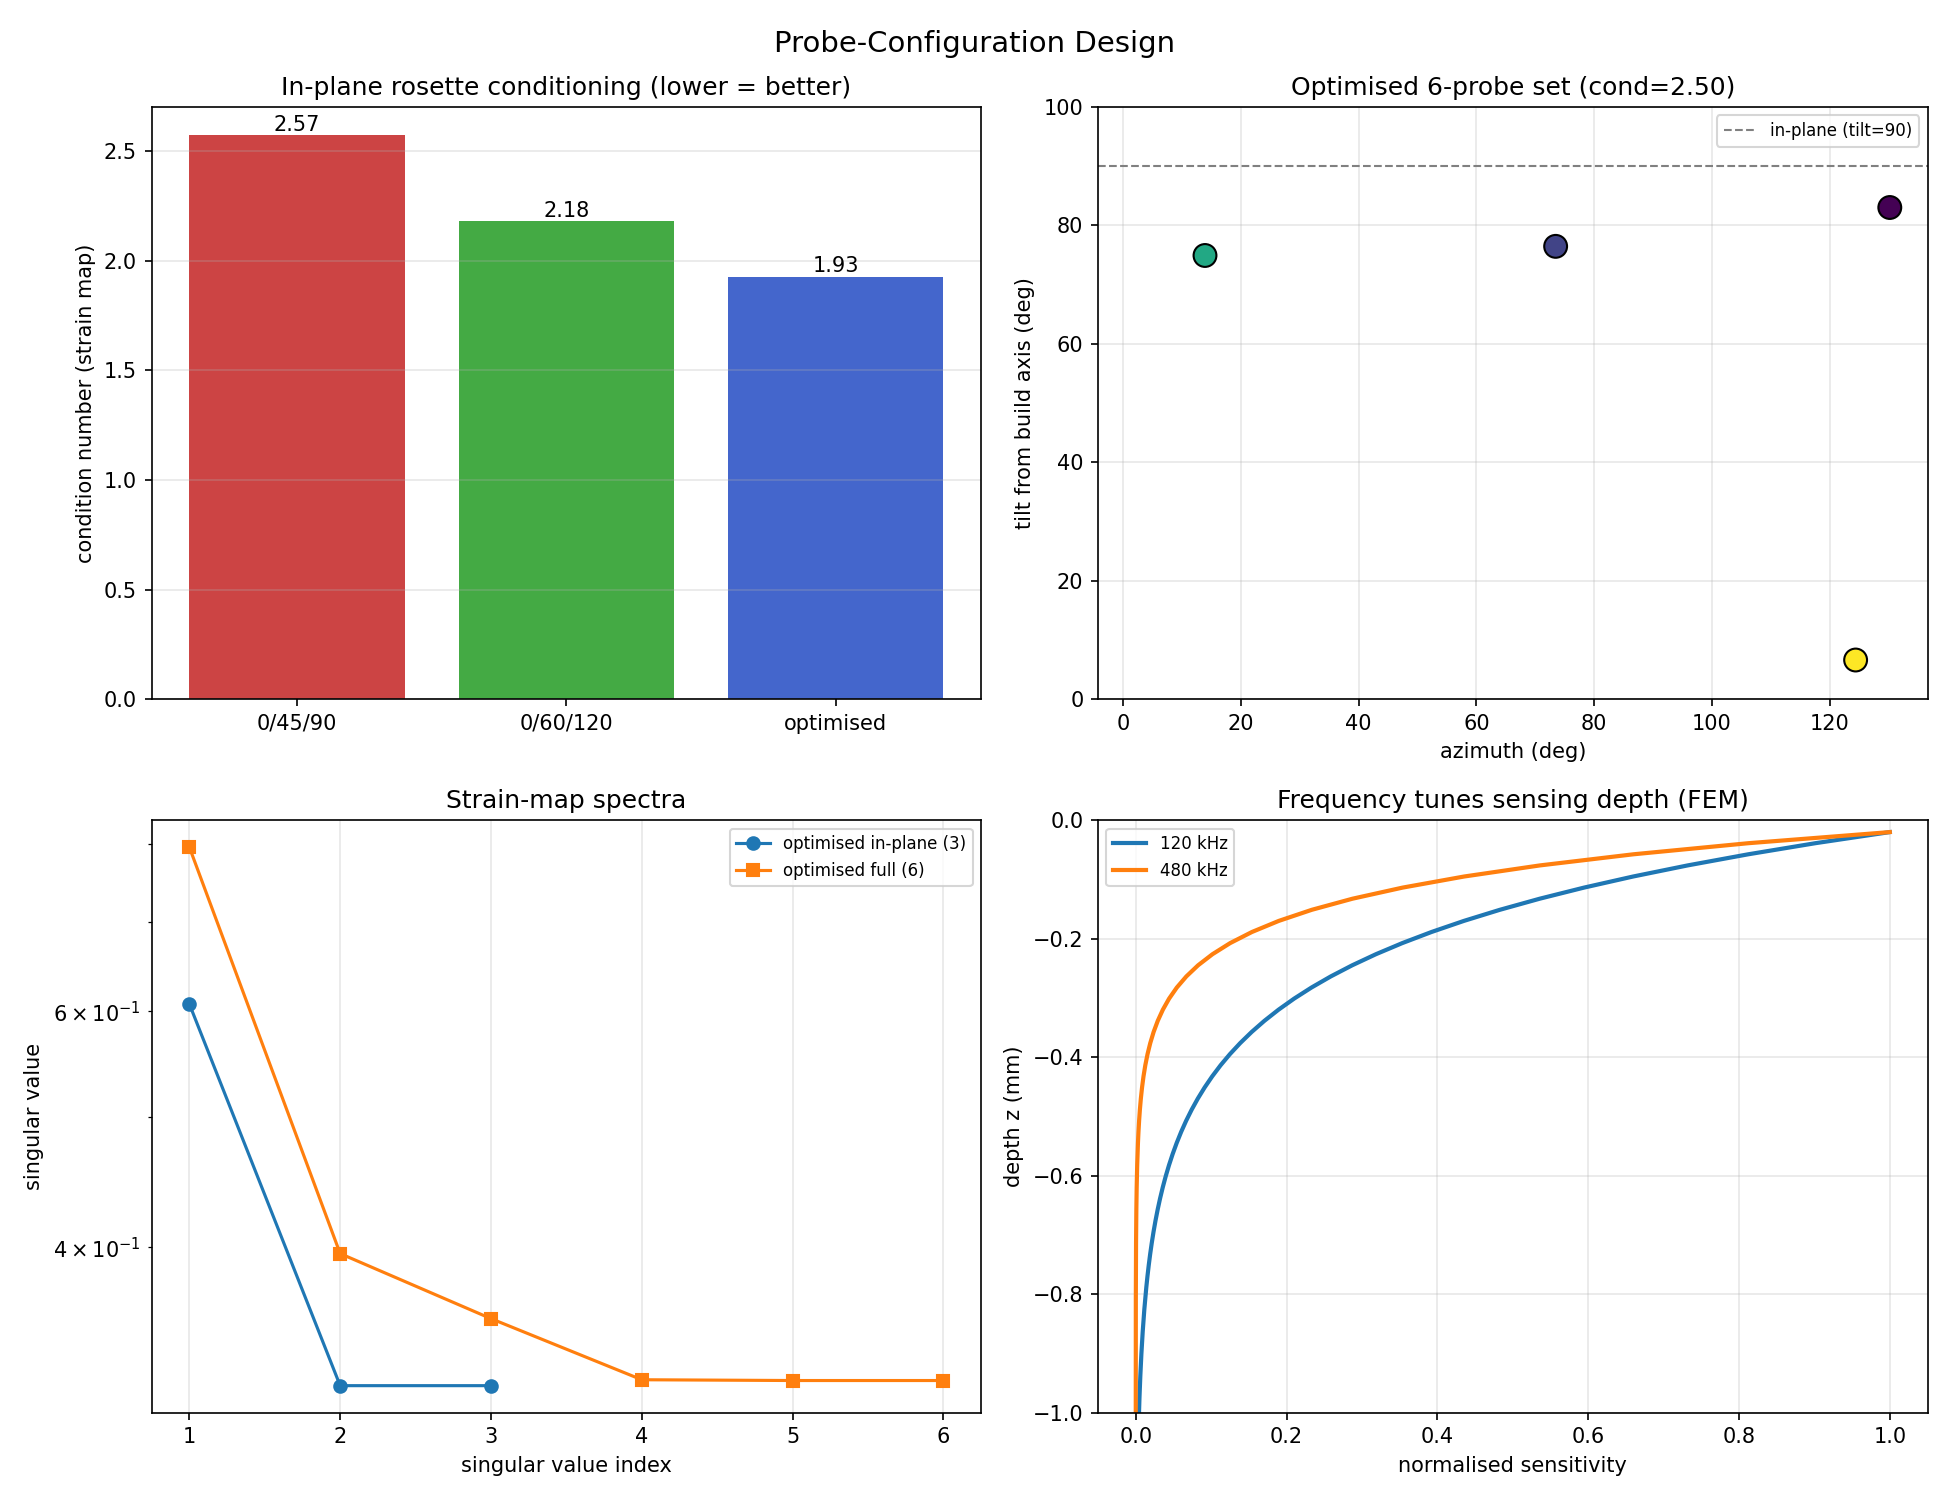
\includegraphics[width=0.92\textwidth]{probe_design_demo.png}
\caption{Probe design. In-plane rosette conditioning (top-left), the optimised
six-probe set in azimuth/tilt (top-right), strain-map spectra (bottom-left), and
the frequency tuning of sensing depth from the FEM model (bottom-right).}
\label{fig:design}
\end{figure}

The ceiling $\operatorname{rank}\Kt$ is itself set by the material.
Figure~\ref{fig:kappa} sweeps the elastoresistivity ratio
$\kappa_\perp/\kappa_\parallel$: the resolvable DOF stay full for any anisotropic
response, but the conditioning of the strain map degrades smoothly toward the
volumetric limit $\kappa_\perp\!\to\!\kappa_\parallel$, where the rank finally
collapses to one. At the thesis-anchored ratio ($\approx0.21$) both the in-plane
rosette and the full set are comfortably conditioned, so the design is
insensitive to the under-determined split between $\kappa_\parallel$ and
$\kappa_\perp$.

\begin{figure}[t]
\centering
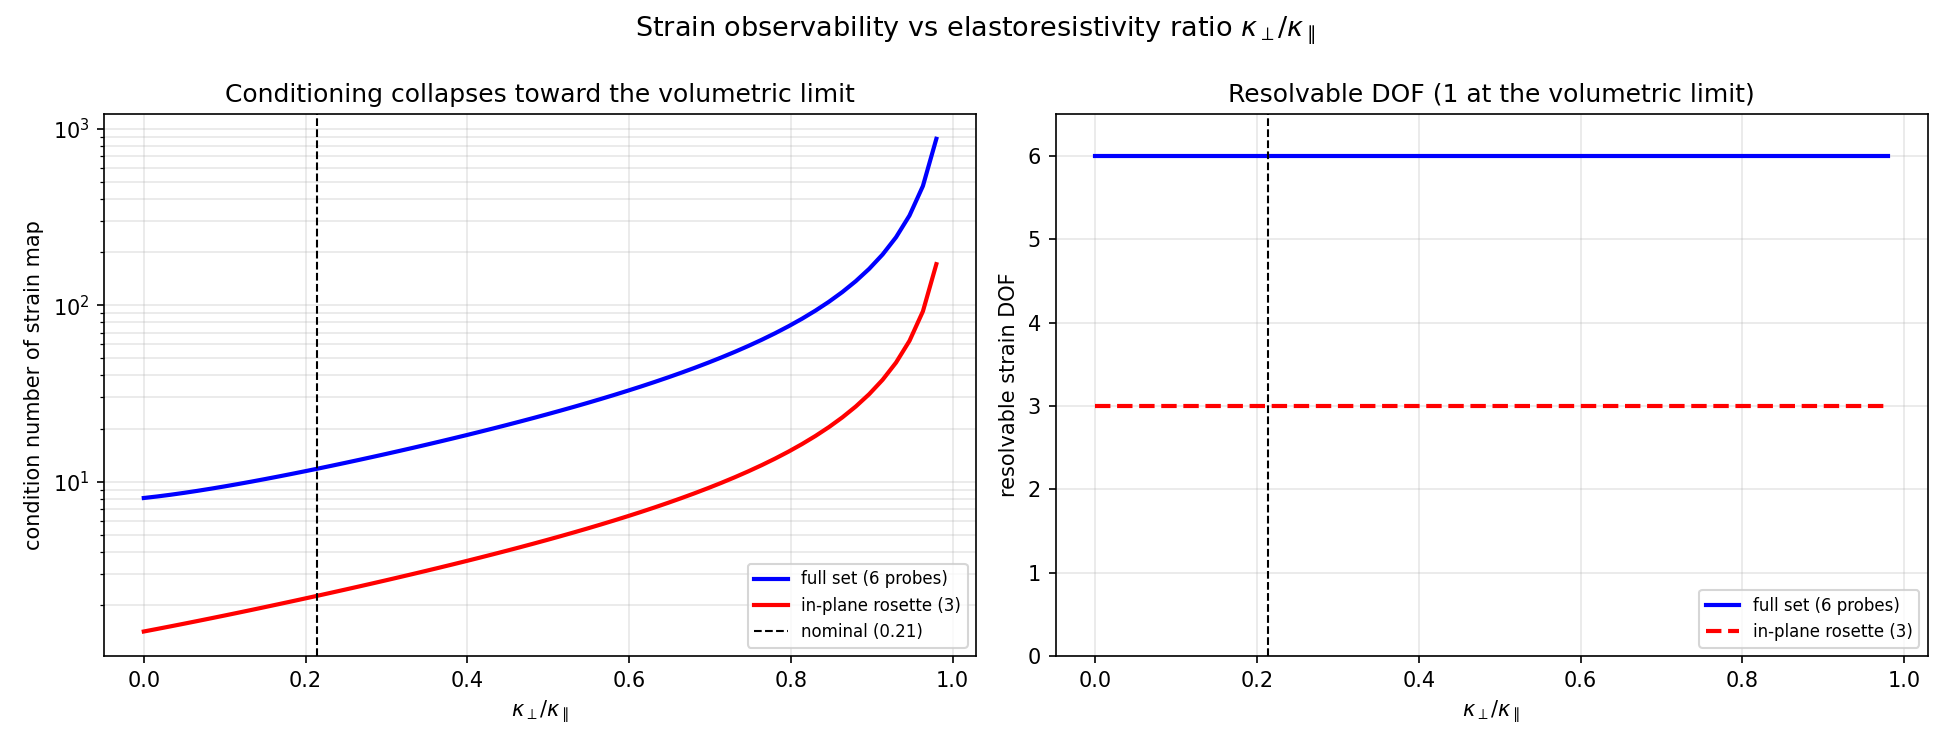
\includegraphics[width=0.92\textwidth]{kappa_sensitivity.png}
\caption{Strain observability vs the elastoresistivity ratio
$\kappa_\perp/\kappa_\parallel$. Left: condition number of the strain map for an
in-plane rosette and a full set, diverging as the response becomes volumetric.
Right: resolvable DOF, full for any anisotropic response. The dashed line marks
the thesis-anchored ratio ($\approx0.21$).}
\label{fig:kappa}
\end{figure}

\section{Tensor-strain inversion with a simulation prior}
\label{sec:inv}
Because realistic probe sets are often rank-deficient (e.g.\ surface access
precludes observing $\sigma_{zz}$), we estimate the strain by maximum a
posteriori (MAP) inversion \cite{aster2018} that fuses measurements with a
process-simulation prior $\eps_{\mathrm{prior}}$ (data assimilation). With
Gaussian measurement noise ($\sigma_d$) and prior ($\sigma_p$),
\begin{equation}
  \eps^\star = \eps_{\mathrm{prior}}
  + \big(\mathsf A^{\!\top}\mathsf A + \lambda \mathsf I\big)^{-1}
  \mathsf A^{\!\top}\big(\bm y - \mathsf A\,\eps_{\mathrm{prior}}\big),
  \qquad \lambda=\sigma_d^2/\sigma_p^2 .
  \label{eq:map}
\end{equation}
The resolution matrix $\mathsf R=(\mathsf A^{\!\top}\mathsf A+\lambda\mathsf
I)^{-1}\mathsf A^{\!\top}\mathsf A$ quantifies, per component, the fraction
supplied by the data (its diagonal): $1$ means measurement-determined, $0$ means
taken from the prior. On a synthetic build-height profile with a deliberately
biased prior, the full set reduces the strain RMSE from $9.4\times10^{-4}$ (prior
only) to $2.6\times10^{-4}$, while the in-plane rosette reaches
$3.9\times10^{-4}$: it corrects the in-plane components from data and falls back
to the prior for $\varepsilon_{zz}$ and the out-of-plane shears, exactly as the
resolution diagonal predicts (Fig.~\ref{fig:inv}). Where only a normal-coil
scalar is available, the estimate degrades gracefully to the volumetric strain
via the invariant coupling $\kappa_v=(\kappa_\parallel+2\kappa_\perp)/3$. The
scalar $\lambda$ here assumes an i.i.d.\ prior and equal probe noise; a full prior
covariance estimated from an ensemble of process simulations, together with an
instrument-referenced impedance-domain noise model, are natural refinements.

\begin{figure}[t]
\centering
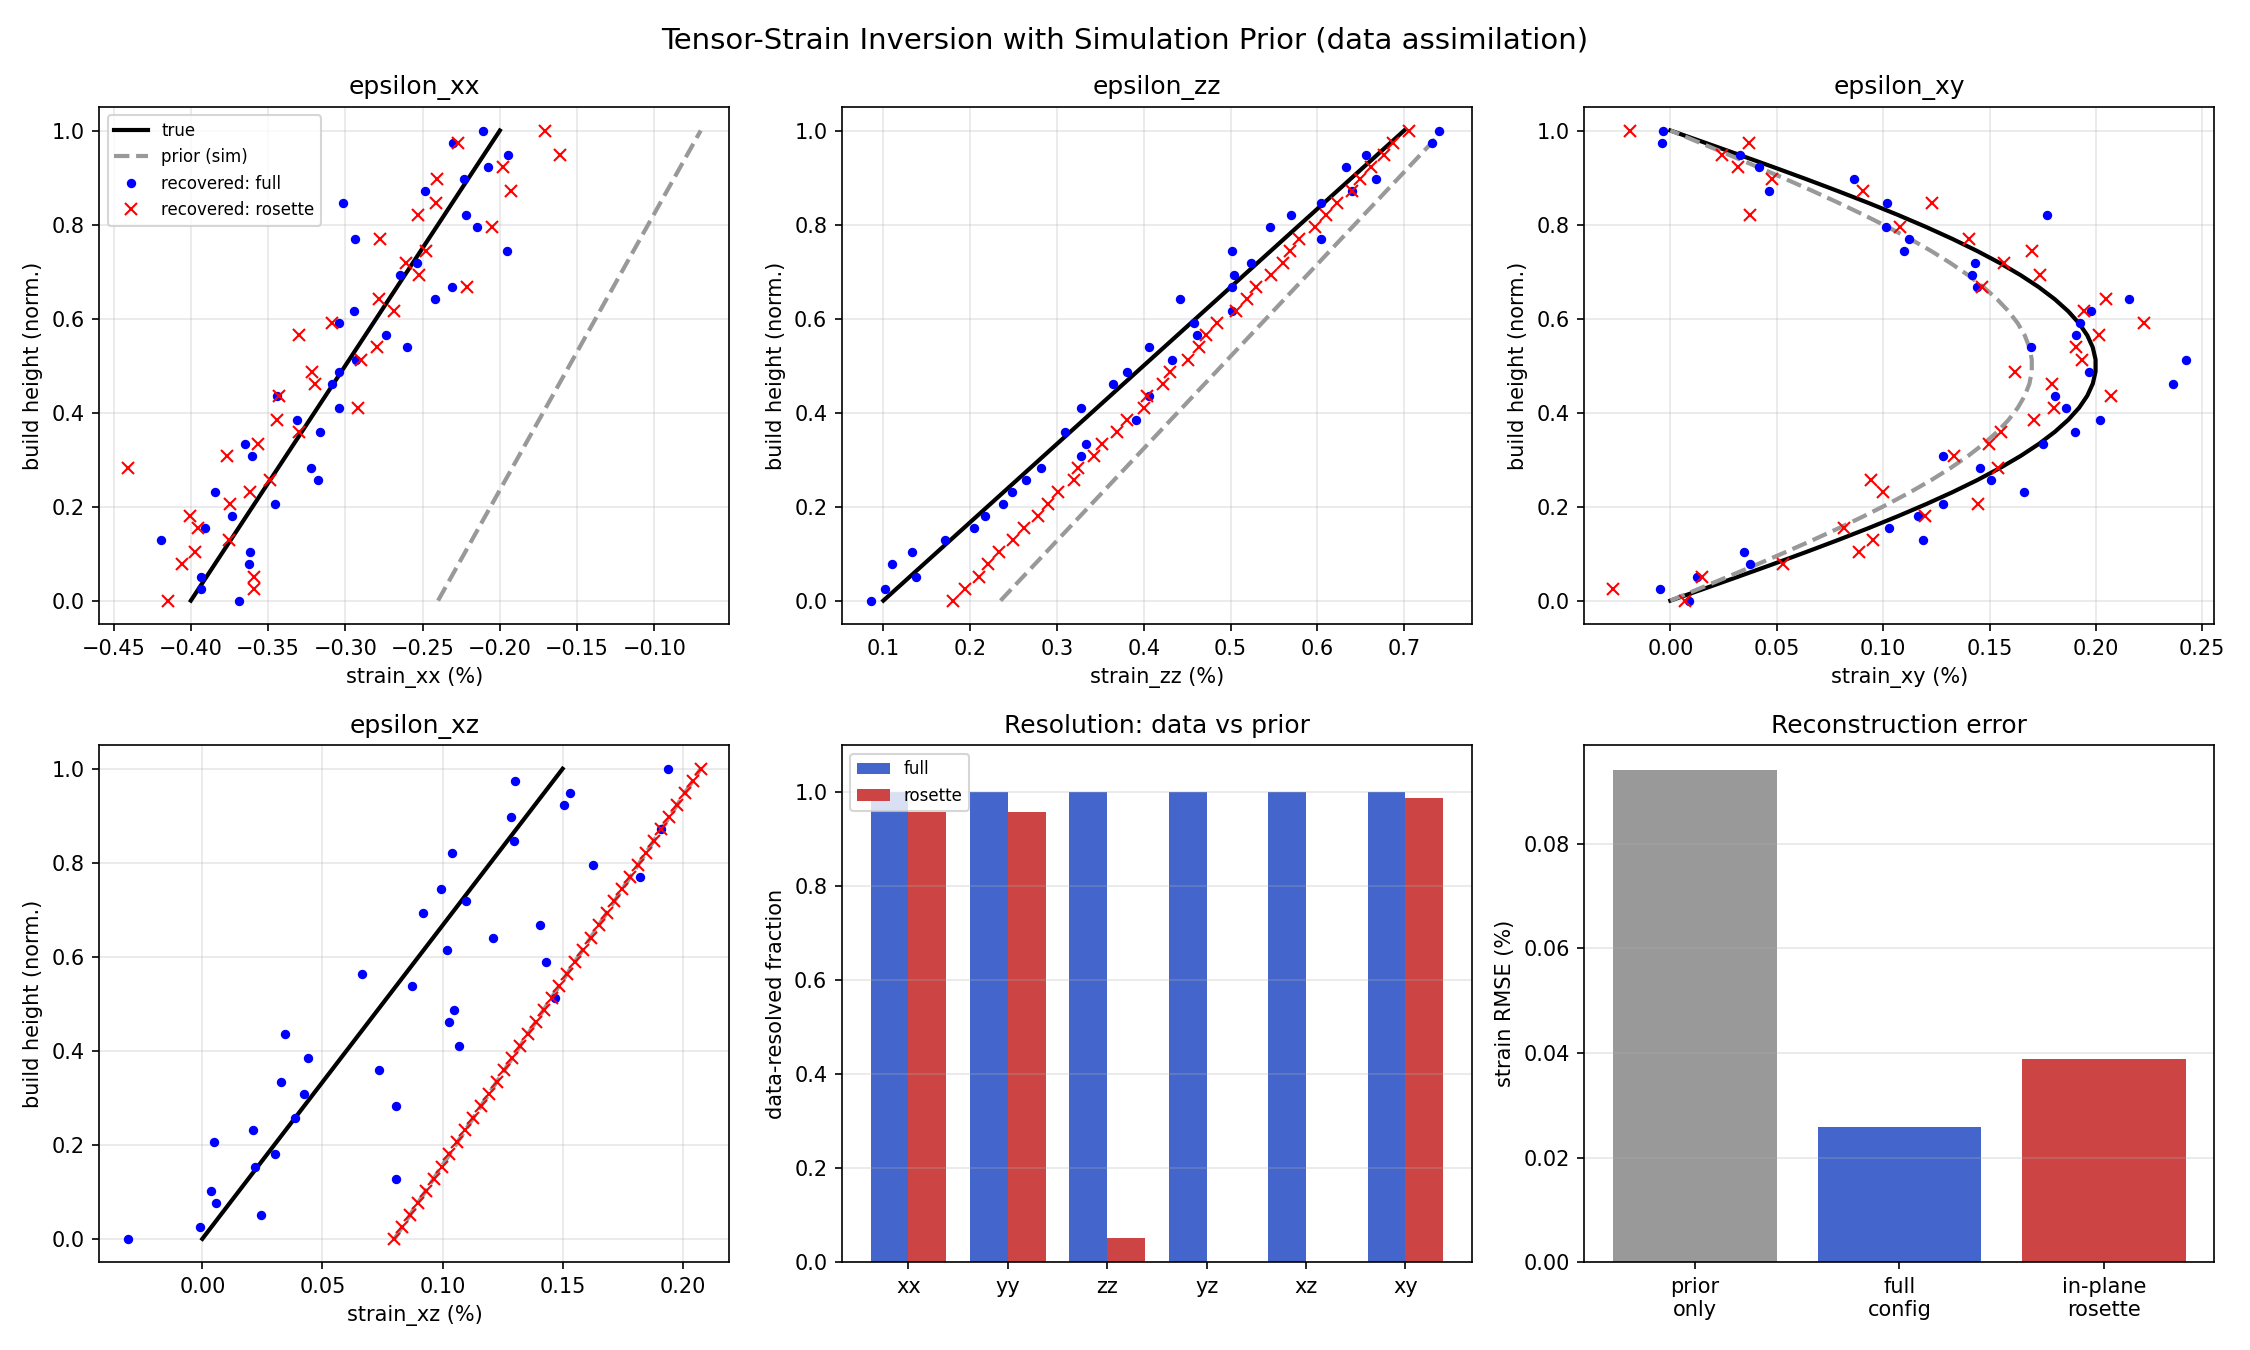
\includegraphics[width=0.92\textwidth]{tensor_inversion_demo.png}
\caption{Tensor-strain inversion with a biased simulation prior. In-plane
components ($\varepsilon_{xx},\varepsilon_{xy}$) are corrected from data by both
configurations; out-of-plane components ($\varepsilon_{zz},\varepsilon_{xz}$) are
recovered only by the full set and otherwise follow the prior, consistent with
the resolution diagonal (centre).}
\label{fig:inv}
\end{figure}

\section{Integrated pipeline}
\label{sec:pipeline}
The forward model, observability, probe design and inversion are combined in a
single open pipeline that ingests layer-wise ECT data and outputs both the
reconstructed geometry (for finite-cell simulation) and, from directional
measurements, a full strain-\emph{tensor} field. Figure~\ref{fig:pipeline} shows
a reconstructed $60\times40\times6$ field for a synthetic build, with the derived
volumetric and von-Mises-equivalent strain fields and the per-component
resolution. Each voxel is currently inverted independently; the finite spatial
footprint of the sensitivity kernel (Fig.~\ref{fig:obs}) couples neighbouring
voxels and should, in a quantitative treatment, be folded into $\mathsf A$ rather
than ignored. The implementation is verified by 66 automated tests.

\begin{figure}[t]
\centering
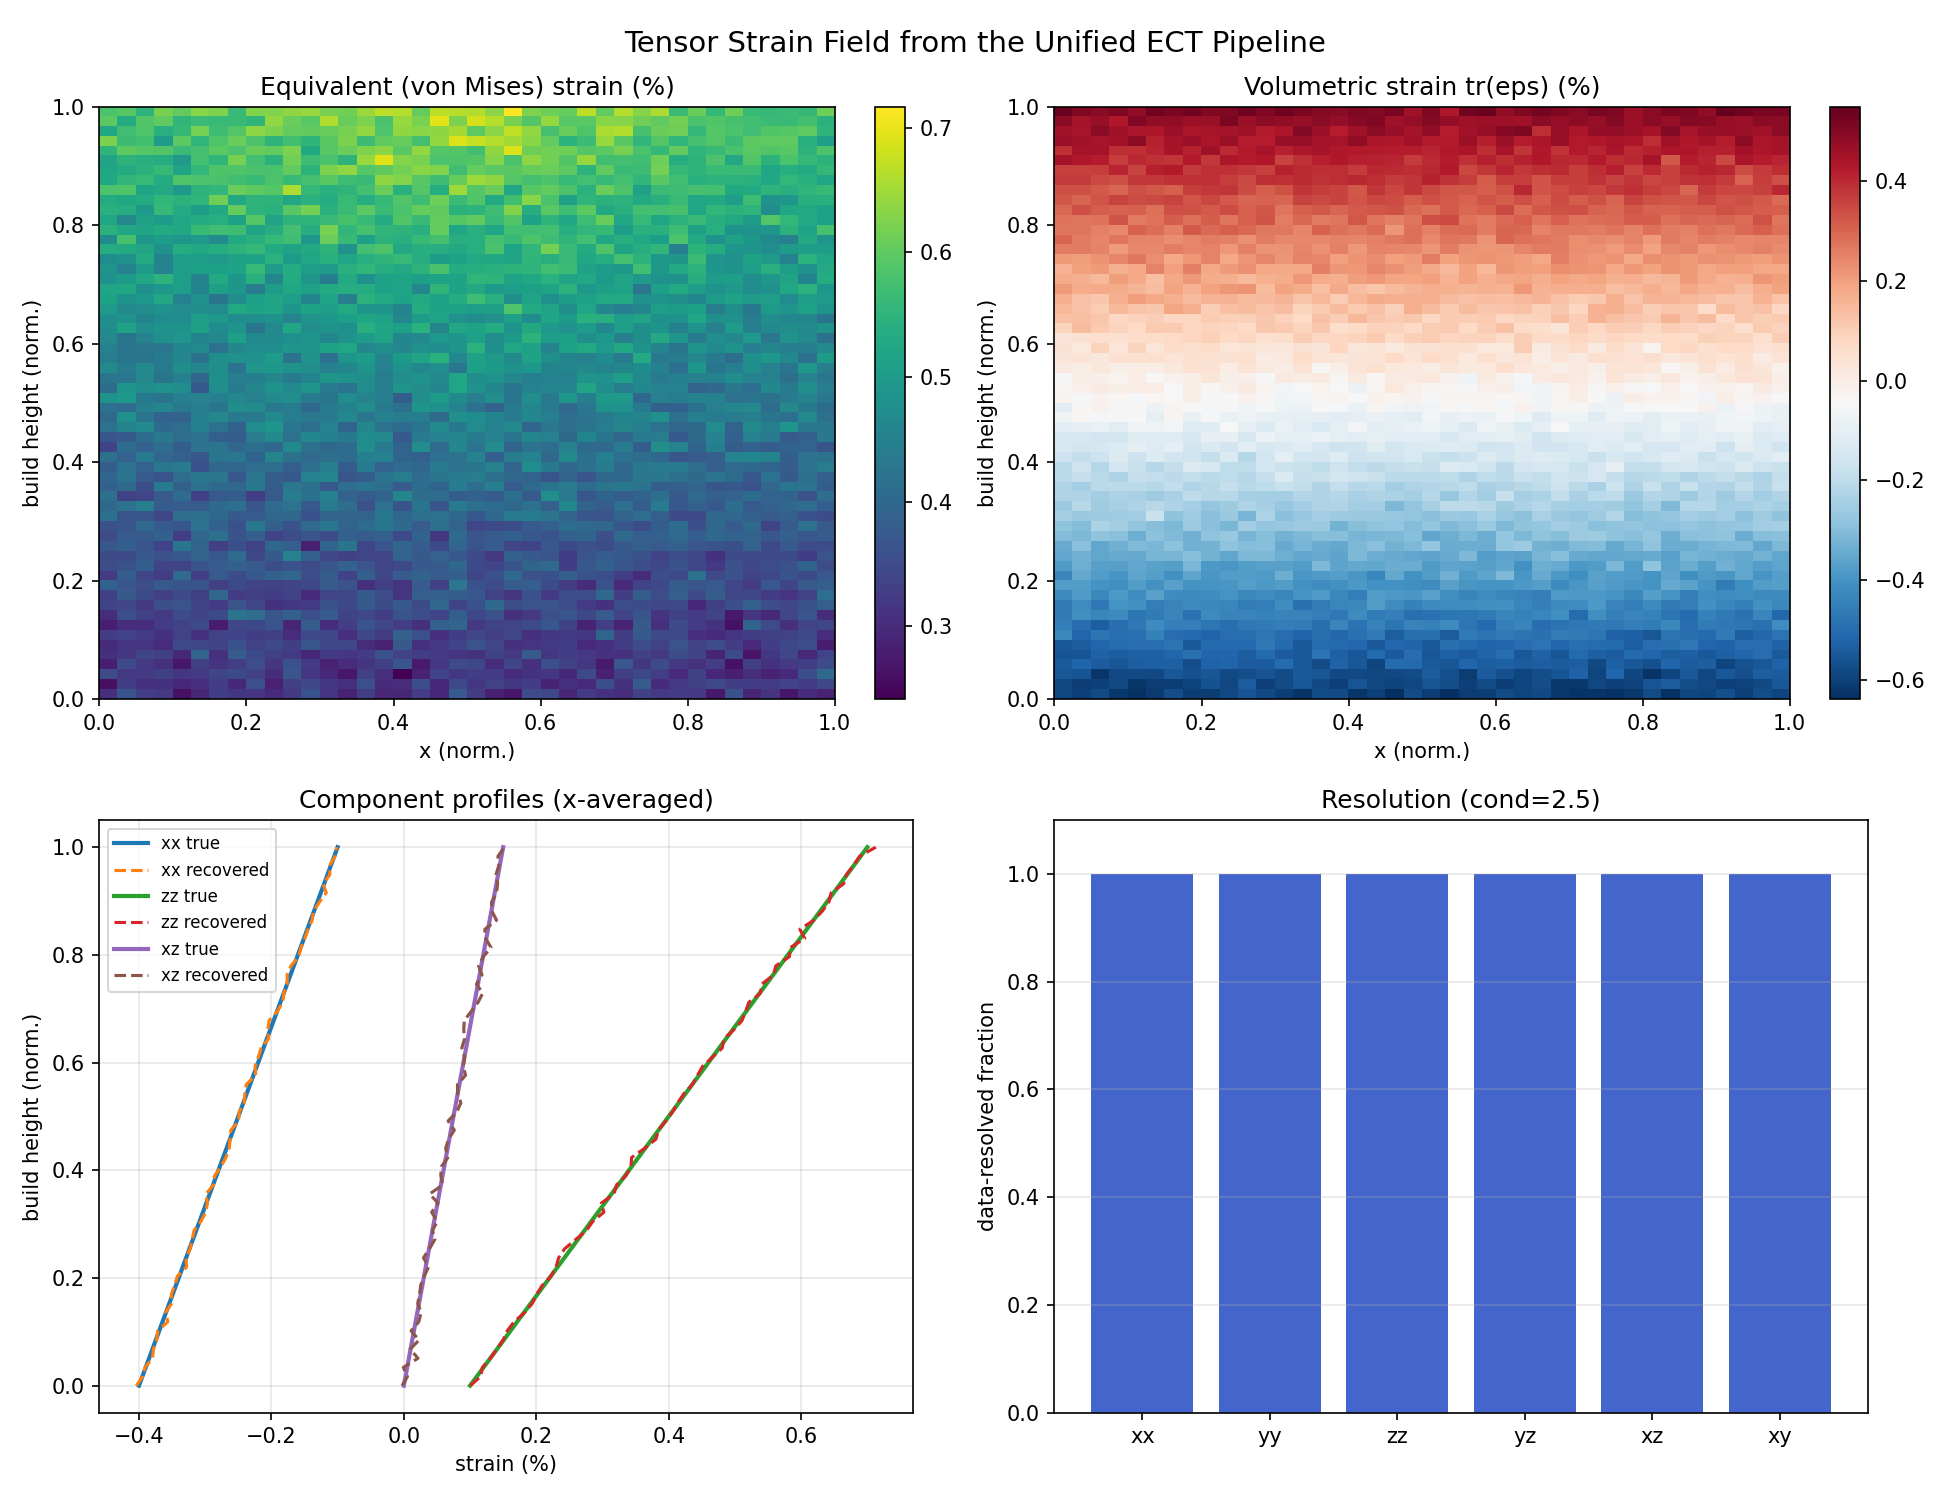
\includegraphics[width=0.92\textwidth]{pipeline_tensor_demo.png}
\caption{Strain-tensor field reconstructed by the unified pipeline. Equivalent
(von Mises) and volumetric strain fields over the build (top), component profiles
versus build height (bottom-left) and the per-component data resolution
(bottom-right).}
\label{fig:pipeline}
\end{figure}

\section{Feasibility: signal, confounders and resolution}
\label{sec:feasibility}
The framework above is geometry- and material-agnostic; deploying it on LPBF 316L
meets three physical realities that set the measurement requirements.

\paragraph{Signal magnitude.} Residual elastic strains in LPBF 316L are of order
$1$--$2\times10^{-3}$, so with $|\kappa|\approx0.33$ the relative conductivity
signal is only $\dsig/\sigma_0\approx3$--$7\times10^{-4}$.

\paragraph{Temperature --- the dominant confounder.} 316L has resistivity
$\rho\approx0.74~\mu\Omega\,$m ($\sigma\approx1.35$~MS/m) with a temperature
coefficient of order $10^{-3}\,$K$^{-1}$ (several $\times10^{-4}\,$K$^{-1}$ near
room temperature) \cite{nist316l}. A drift of only ${\sim}1$~K therefore changes
$\sigma$ by as much as the entire strain signal --- consistent with in-situ ECT
studies that found part temperature dominant and required explicit compensation
\cite{spurek2024}. Strain sensing thus demands differential or reference-channel
probes, multi-frequency lift-off/temperature separation, and tight thermal
referencing. Cold work and dislocation density (Section~1) are a further,
microstructure-borne confounder that co-varies with the thermal history.

\paragraph{Penetration and depth resolution.} At the realistic 316L conductivity
the skin depth is $\delta=\sqrt{2/(\omega\mu\sigma)}\approx0.9$~mm at $240$~kHz
(falling to ${\approx}0.4$~mm at $1$~MHz), far larger than a $30$--$50~\mu$m
layer: each measurement averages roughly $20$--$30$ deposited layers. The
$60\times40\times6$ reconstruction of Section~\ref{sec:pipeline} is therefore a
coarse-$z$ illustration; layer-resolved tomography would require multi-frequency
depth inversion, and the forward-model benchmark of Table~\ref{tab:fem} (a higher,
generic conductivity, $\delta\approx0.25$~mm) should be read as a verification
case rather than a 316L prediction.

These constraints do not undermine the framework --- they specify the instrument:
a thermally-referenced, multi-frequency directional-probe rosette, whose
observability and conditioning are exactly what
Sections~\ref{sec:obs}--\ref{sec:design} quantify.

\section{Discussion}
The cross-validation between the analytical and FEM forward models proved
unexpectedly valuable, exposing two independent errors in a widely used
analytical formulation (a reflection-coefficient sign and a units error in the
propagation parameter) that a self-consistent synthetic round trip would never
reveal; after correction the two models agree to within $1\%$ in resistance and
$3\%$ in reactance. This underlines the importance of dissimilar, redundant
forward models when an inverse method is to be trusted on real data.

Two limitations frame the path to experiment. First, surface ECT accesses
in-plane current paths much more readily than out-of-plane ones, so
$\varepsilon_{zz}$ and the out-of-plane shears will in practice lean on the
simulation prior or on multi-frequency depth profiling; edge access or tilted
probes mitigate this. Second, the tensor model needs calibration:
multi-orientation tensile tests are required to populate
$\kappa_\parallel,\kappa_\perp$ (and the as-built anisotropy of $\sigma_0$ in
columnar LPBF microstructures).

\section{Conclusion}
We have shown how to progress from a scalar strain--conductivity relation to a
tensorial reconstruction with ECT. The key realisation is that the scalar
impedance constrains a \emph{projection} of the conductivity tensor; resolving
the strain tensor then requires measurement diversity (a directional/tilted probe
``rosette'', optionally multi-frequency) and, for the components that remain
unobservable, a physics-based prior fused by regularised inversion. The framework
is fully implemented and verified, and --- as a by-product of cross-validating
two dissimilar forward models --- caught two implementation pitfalls in our
realisation of the classical model (a reflection sign and a units error in the
propagation parameter), after which the two models agree to $0.9\%$ in
resistance. Future work targets a 3-D anisotropic eddy-current model to quantify
the true out-of-plane sensitivity of tilted and elongated probes, experimental
calibration of the elastoresistivity constants, and deployment of the pipeline
for in-situ monitoring.

\section*{Code and data availability}
The open-source pipeline (forward models, observability, probe design and
inversion) and the scripts that regenerate every figure are available at
\url{https://github.com/MassimoCarraturo/eddy_current_project}; an archived
release with a DOI will be deposited on Zenodo.

\section*{CRediT author statement}
\textbf{M.\ Carraturo:} conceptualisation, methodology, software, writing ---
original draft. \textbf{B.\,I.\ Ates:} calibration data, methodology, writing ---
review and editing.

\section*{Declaration of generative AI}
Generative-AI tools assisted software development and manuscript editing; all
scientific content was verified by the authors, who take full responsibility for
it. AI tools are not listed as authors.

% NOTE (draft): volume/issue/page details for several entries should be
% completed before submission; entries below are author/title/venue/year-verified.
\begin{thebibliography}{99}
\bibitem{dodd1968} C.\,V.\ Dodd, W.\,E.\ Deeds. Analytical solutions to
eddy-current probe-coil problems. \emph{J.\ Appl.\ Phys.}\ 39(6):2829--2838, 1968.
\bibitem{bowler2019} J.\,R.\ Bowler. \emph{Eddy-Current Nondestructive
Evaluation}. Springer, 2019.
\bibitem{auld1999} B.\,A.\ Auld, J.\,C.\ Moulder. Review of advances in
quantitative eddy current nondestructive evaluation. \emph{J.\ Nondestruct.\
Eval.}\ 18:3--36, 1999.
\bibitem{theodoulidis2006} T.\,P.\ Theodoulidis, E.\,E.\ Kriezis. \emph{Eddy
Current Canonical Problems (with Applications to Nondestructive Evaluation)}.
Tech Science Press, 2006.
\bibitem{garcia2011} J.\ Garc\'ia-Mart\'in, J.\ G\'omez-Gil,
E.\ V\'azquez-S\'anchez. Non-destructive techniques based on eddy current
testing. \emph{Sensors}\ 11(3):2525--2565, 2011.
\bibitem{yu2004} F.\ Yu, P.\,B.\ Nagy. Eddy current assessment of near-surface
residual stress in shot-peened nickel-base superalloys. \emph{J.\ Nondestruct.\
Eval.}\ 23(1), 2004.
\bibitem{abunabah2006} B.\,A.\ Abu-Nabah, P.\,B.\ Nagy. Iterative inversion
method for eddy current profiling of near-surface residual stress in
surface-treated metals. \emph{NDT\&E Int.}, 2006.
\bibitem{abunabah2007} B.\,A.\ Abu-Nabah, P.\,B.\ Nagy. High-frequency eddy
current conductivity spectroscopy for residual stress profiling in
surface-treated nickel-base superalloys. \emph{NDT\&E Int.}, 2007.
\bibitem{spurek2022} M.\,A.\ Spurek et al. In-situ monitoring of powder bed
fusion of metals using eddy current testing. \emph{Additive Manufacturing}, 2022.
\bibitem{spurek2024} M.\,A.\ Spurek et al. Influence of part temperature on
in-situ monitoring of powder bed fusion of metals using eddy current testing.
\emph{Progress in Additive Manufacturing}, 2024.
\bibitem{monu2025} M.\,C.\,C.\ Monu, J.\,C.\ Chekotu, D.\ Brabazon. Eddy current
testing and monitoring in metal additive manufacturing: a review. \emph{J.\
Manuf.\ Process.}, 2025.
\bibitem{bartlett2019} J.\,L.\ Bartlett, X.\ Li. An overview of residual stresses
in metal powder bed fusion. \emph{Additive Manufacturing}\ 27:131--149, 2019.
\bibitem{withers2001} P.\,J.\ Withers, H.\,K.\,D.\,H.\ Bhadeshia. Residual stress.
Part 1 --- measurement techniques. \emph{Mater.\ Sci.\ Technol.}\
17(4):355--365, 2001.
\bibitem{nist316l} Measurements of thermophysical properties of solid and liquid
NIST SRM~316L stainless steel. National Institute of Standards and Technology,
2021.
\bibitem{ates2025} B.\,I.\ Ates. \emph{Towards Eddy Current-Based Strain
Prediction in Laser Powder Bed Fusion of Metals}. MSc thesis, Technical
University of Munich, 2025.
\bibitem{aster2018} R.\,C.\ Aster, B.\ Borchers, C.\,H.\ Thurber. \emph{Parameter
Estimation and Inverse Problems}, 3rd ed. Elsevier, 2018.
\end{thebibliography}

\end{document}
